% !TeX program = xelatex
% !BIB program = biber

\documentclass[a4paper]{article}

\usepackage{longtable}
\usepackage{array}
\usepackage{placeins}
\usepackage{csquotes}
\usepackage{hyperref}
\usepackage{graphicx}
\usepackage{url}
\usepackage{todonotes}
\usepackage{booktabs}
\usepackage{tablefootnote}
\usepackage{siunitx}
\usepackage{multirow}
\usepackage{tabularx}
\sisetup{output-exponent-marker=\ensuremath{\mathrm{e}}}
\usepackage[english, german, ngerman]{babel}
\usepackage[
    backend=biber,
    style=apa,
    autocite=inline,
    mincitenames=1,
    maxcitenames=2
]{biblatex}

\addbibresource{thesis-literature.bib}
\addbibresource{thesis-software.bib}
\addbibresource{thesis-online.bib}



\selectlanguage{ngerman}

\def\UrlFont{\rmfamily}

\begin{document}

\begin{titlepage}
    \begin{center}
        \vspace*{1cm}

        \textbf{\Large Automatisierte Erkennung von verschwörungstheoretischen Artikeln}

        \vspace{0.5cm}
        Mit Methoden der natürlichen Sprachverarbeitung und des maschinellen Lernens
                
        \vspace{1.5cm}


        \vfill
                
        Bachelor-Arbeit zur Erlangung des akademischen Grades eines\\
        B.Sc. Digital Humanities

        \vspace{3cm}
                
        Eingereicht von: David Fuhry
        
        \vspace{0.2cm}

        Matrikel-Nr. 3704472\\
        Zschochersche Str. 32\\
        04229 Leipzig

        \vspace{1cm}

        Betreuer: Jun.-Prof. Dr. Phil. Manuel Burghardt
        
        \vspace{0.2cm}
                    
        Computational Humanities\\
        Institut für Informatik\\
        Universität Leipzig\\
        Augustusplatz 10\\
        04109 Leipzig 
                
    \end{center}
\end{titlepage}

\tableofcontents

\thispagestyle{empty}

\newpage

% Introduction

\pagenumbering{arabic}

\section{Einleitung}

Verschwörungstheorien sind aktuell häufig im Zentrum der öffentlichen Aufmerksamkeit.
Während dieser Aufmerksamkeitsschub vor allem auf die Covid-19 Pandemie zurückzuführen ist, erleben Verschwörungstheorien schon seit Anfang der 2000er Jahre einen Popularitätsanstieg.
Dieser ist vor allem begründet in der zunehmenden Verbreitung des Internets und der sozialen Medien \parencite[vgl.][492]{stano_2020}.

Eine der Kernfragen in der wissenschaftlichen Auseinandersetzung mit Verschwörungstheorien ist die Frage was eine Verschwörungstheorie ist und was nicht.
Eine theoretische Auseinandersetzung mit dieser Frage findet insbesondere in der Wissensoziologie und der Philosophie statt.\footnote{Siehe z.B. \textcite[]{coady_2006} oder auch \textcite{uscinski_2014}.}
Weitgehend unbeantwortet ist hingegen wie sich diese Frage quantitativ beantworten lässt.
Die wenigen hierzu veröffentlichten Arbeiten nutzen meist verhältnismäßig spezifische und komplexe Methoden.\footnote{Siehe etwa \textcite[]{samory_2018} oder \textcite[]{shahsavari_2020}.}

Diese Arbeit stellt einen Ansatz vor, der versucht dieses Problem mit Methoden des Text-Mining und des maschinellen Lernens zu lösen.
Der vorgestellte Ansatz ist dabei deutlich allgemeiner als die in der Literatur vertretenen und versucht verschwörungstheoretische Texte mittels sprachlicher und stilistischer Merkmale zu identifizieren.

Es wird dafür ein Korpus aus Artikeln von 7 Webportalen der deutschsprachigen, verschwörungstheoretischen Szene ausgewertet. 
Aus diesem werden Features extrahiert, die anschließend genutzt werden um ein Modell zu trainieren, welches diese Artikel von (wissenschafts-)journalistischen Artikeln unterscheiden kann.
Dabei erfolgt ein Rückgriff auf in der bestehenden, überwiegend qualitativen Forschung gemachte Erkenntnisse und Beobachtung.
Auch werden Methoden aus der natürlichen Sprachverarbeitung verwendet um Features aus Wortfrequenzen und Part-of-Speech Tags zu erstellen.

Das erstellte Modell kann präzise verschwörungstheoretische Artikel identifizieren und von denen im Vergleichskorpus unterscheiden.
Die dabei gemachten Beobachtungen können dabei helfen in der qualitativen Forschung gemachte Beobachtungen quantitativ zu validieren.
Auch könnte die hier vorgestellte Methode hilfreich sein um verschwörungstheoretische Inhalte in größeren Datenmengen zu identifizieren.

% Theorie

\section{Theoretische Perspektiven}

\subsection{Forschungsstand zu Verschwörungstheorien}

Das Erscheinen von Richard Hofstadters Essay \textit{The Paranoid Style in American Politics} \parencite[][]{hofstadter_2008} wird heute üblicherweise als der Beginn der modernen wissenschaftlichen Auseinandersetzung mit Verschwörungstheorien betrachtet.
In seiner Arbeit setzt Hofstadter sich mit dem Einfluss von Verschwörungstheorien und konspirativer Rhetorik (dem \textit{Paranoid Style}) auf die US-amerikanische Politik auseinander.
Ein Beispiel auf das Hofstadter eingeht, sind die Schriften von Senator McCarthy und die nach ihm benannte Praxis des McCarthyismus.

Das weitere Forschungsinteresse im restlichen 20. Jahrhundert war eher gering, die verbleibende Forschung fiel meist in eine von zwei Kategorien, wie \textcite{sunstein_2008} passend zusammenfassen:

\begin{quotation}
    The academic literature on conspiracy theories is thin, and most of it falls into one 
    of two classes: (1) work by analytic philosophers, especially in epistemology and the 
    philosophy of science, that asks what counts as a “conspiracy theory” and whether such theories are methodologically suspect; (2) a smattering of work in sociology and Freudian psychology on the causes of conspiracy theorizing. \parencite[][2]{sunstein_2008}
\end{quotation}

In der jüngeren Vergangenheit haben mehrere Entwicklungen Verschwörungstheorien und damit auch der Forschung in diesem Bereich Vorschub geleistet.

Dies war zum einen die zunehmende Verbreitung des Internets um die Jahrtausendwende.
Die Mehrheit der Autor:innen sieht darin ein erhebliches Hilfsmittel für die Verbreitung von Verschwörungstheorien.
So schreibt etwa \textcite{stano_2020}: "[...] The Internet, and in particular social networks, have proved fundamental to the spread and development of such [conspiracy] theories" \parencite[][492]{stano_2020}.\footnote{Es gilt jedoch anzumerken, dass auch die gegenteile Auffassung in der Literatur vertreten ist, etwa bei \textcite{clarke_2007}.}

In der jüngsten Vergangenheit haben insbesondere die Wahl Donald Trumps zum US-Präsidenten im Jahr 2016 und die aktuelle Covid-19 Pandemie Verschwörungstheorien in das allgemeine Bewusstsein gerückt.
Während die wissenschaftliche Aufarbeitung, insbesondere der mit der Covid-19 Pandemie einhergehenden Welle an Verschwörungstheorien, noch am Anfang steht, sind bereits erste Arbeiten entstanden, die neue, vielversprechende Ansätze zeigen, wie etwa von \textcite{shahsavari_2020}.

Eines der Kernprobleme in der Arbeit mit Verschwörungstheorien ist es, diese verlässlich als solche zu identifizieren.
Dies hat nicht nur eine fundamentale Rolle für theoretische Arbeiten, sondern ist auch von immenser praktischer Relevanz, ist die Grenze zwischen Verschwörungstheorien und Nachrichten in den sozialen Medien doch zunehmend schwerer auszumachen.

In der Vergangenheit war die wissenschaftliche Beantwortung dieser Frage meist eng mit der Frage danach verbunden, was eine Verschwörungstheorie konstituiert und anhand welcher Kriterien sich dies erfassen lässt.
Eine beispielhafte Arbeit ist zu finden bei \textcite{uscinski_2014}.
Die Autor:innen nutzen darin sechs verschiedene Tests um Verschwörungstheorien zu identifizieren. Als Beispiel seien Occam's razor, also die Frage nach der einfachsten Erklärung, und die Falsifizierbarkeit einer Theorie genannt.
In der Arbeit wird mit diesen Kriterien und der Methode der Inhaltsanalyse, sowie einer Vielzahl von studentischen Kodierer:innen, ein Korpus aus Briefen an US-Redaktionen ausgewertet \parencite[54ff]{uscinski_2014}.
Während die Autor:innen überzeugend dafür argumentieren, alle der aufgestellten Kriterien für eine Klassifizierung einzusetzten \parencite[52f]{uscinski_2014}, ist keines der eingeführten Kriterien wirklich geeignet um automatisierte Klassifikationen vorzunehmen, zumindest mit den aktuellen technischen Möglichkeiten.

In der jüngeren Vergangenheit sind demgegenüber erste Arbeiten entstanden, die sich mit automatisieren Verfahren rund um Verschwörungstheorien beschäftigen.
Eine solche Arbeit ist die von \textcite{samory_2018}, in der die Autor:innen automatisiert Triplets bestehend aus \textit{agent}, \textit{action} und \textit{target} aus verschwörungstheoretischen Online-Kommentaren extrahieren.
Als Datengrundlage nutzen sie dazu Beiträge aus dem Reddit Subforum r/conspiracy.
Diese werten sie mittels einer NLP-Pipeline aus, die unter anderem Topic Modeling, Dependency Parser und Wortvektoren nutzt, aber auch vereinzelt menschliche Expertise einbringt \parencite[][6ff]{samory_2018}.
Der Ansatz stellt einen wichtigen Beitrag zu einer vollständig automatisierten Analyse dar, ist aber auch verhältnismäßig komplex und benötigt Eingriffe durch menschliche Expert:innen.

Eine weitere Arbeit, die sich mit automatisierten Auswertungen beschäftigt, ist die von \textcite{shahsavari_2020}.
Die Autor:innen werten darin Online-Diskussionen zur Covid-19 Pandemie in Foren wie Reddit und 4Chan aus.
Die Auswahl der Beiträge mit verschwörungstheoretischem Inhalt, wurde dabei von einem Expert:innengremium getroffen \parencite[284f]{shahsavari_2020}.
Es werden, mittels Methoden aus der natürlichen Sprachverarbeitung, narrative Netzwerke ausgewertet und so Verbindungen zu den Inhalten von Nachrichten und den aktuell populärsten Verschwörungstheorien aufgezeigt.

Näher an der Problemstellung dieser Arbeit ist die Methode die von \textcite{potthast_2018} vorgestellt wird.
Darin nutzen die Autor:innen Methodik um mit Verfahren des maschinellen Lernens und stilistischen Features Fake-News und politisch extreme Artikel zu identifizieren.
Sie greifen dabei auf einen von professionellen Journalist:innen kategorisierten Korpus zurück und können Artikel aus politisch extremen Quellen mittels dieser Merkmale von anderen unterscheiden.
Da Verschwörungstheorien eine Schnittmenge mit Fake-News und insbesondere der rechtsextremen Szene haben \parencite[vgl.][]{stumpf_2019}, könnte dieser Ansatz auch für die Identifizierung verschwörungstheoretischer Inhalte relevant sein.

\subsection{Stilistische Merkmale verschwörungstheoretischer Texte}

Um Verschwörungstheorien zuverlässig zu identifizieren, soll zunächst ein Blick in die Literatur erfolgen und auf die in der qualitativen und quantitativen Forschung gemachten Beobachtungen zu sprachlichen Merkmalen von Verschwörungstheorien.
Eine erschöpfende Auflistung aller in der Literatur zu findenden sprachlichen Merkmale von Verschwörungstheorien ist, insbesondere mit dem erstarkten Forschungsinteresse in der jüngsten Vergangenheit, kaum möglich, noch wäre sie zielführend.
Es sollen daher hier vor allem solche Merkmale genannt werden, die sich potenziell für eine quantitative, automatisierte Erfassung eignen.

Eine in der Literatur häufig gemachte Beobachtung ist die Emotionalität der Argumentation in Verschwörungstheorien \parencite[vgl.][10]{miller_2002}.
Dieses Merkmal findet sich auch bei \textcite[][93ff]{butter_2018}, der noch spezifischer darauf eingeht, dass es vor allem die vermeintlichen Verschwörer sind, denen mit "metaphorisch aufgeladener, bisweilen apokalyptischer Sprache ausschließlich negative Eigenschaften zugeschrieben [werden]" \parencite[][93f]{butter_2018}.

Während die Emotionalität spezifischer Aspekte der Argumentation eine häufig gemachte Beobachtung ist, steht dazu im Gegensatz die Beobachtung über den allgemeinen Stil der Verschwörungstheoretiker:innen.
So spricht ebenfalls \textcite[][61]{butter_2018} davon, dass sich Verschwörungstheoretiker traditionell um eine seriöse Darstellung bemühen und sich der verwendete Stil an dem der Wissenschaft anlehne.
Diese Feststellung findet sich bereits bei \textcite{hofstadter_2008}:

\begin{quotation}
    The higher paranoid scholarship is nothing if not coherent—in fact the paranoid mind is far more coherent than the real world. It is nothing if not scholarly in technique. McCarthy’s 96-page pamphlet, McCarthyism, contains no less than 313 footnote references, and Mr. Welch’s incredible assault on Eisenhower, The Politician, has one hundred pages of bibliography and notes. \parencite[][37]{hofstadter_2008}
\end{quotation}

Seit der Erstveröffentlichung von Hofstadters Essays hat vor allem die Verbreitung des Internets zu Veränderungen in der Erzählart von Verschwörungstheorien geführt.
Die Obsession an Belegen und Referenzen existiert zwar weiterhin, hat sich aber insoweit verändert, als das nicht mehr unbedingt Fußnoten das Mittel der Wahl sind.
Vielmehr wird sich der Möglichkeiten des Internets bedient, Inhalte direkt einzubinden oder zu verlinken.
So schreibt etwa \textcite{soukup_2008}, der sich spezifisch mit Verschwörungstheorien um den 11. September befasst, diese müssten als "digital, hypertextual, and multimedial experience" \parencite[10]{soukup_2008} verstanden werden.

Erst in der jüngeren Vergangenheit finden sich Arbeiten die sich spezifisch mit den linguistischen Merkmalen von Verschwörungstheorien auseinandersetzen.
\textcite{schafer_2018} etwa analysiert einen Korpus aus Kommentaren zu verschwörungstheoretischen YouTube-Videos.
Sie stellt dabei unter anderem eine gehäufte Verwendung von Ironie und scare quotes fest, insbesondere dann, wenn es darum geht die Gegenseite negativ darzustellen \parencite[235]{schafer_2018}.
Ähnlich der bereits erörterten Literatur findet die Autorin auch eine hohe Dichte von Belegen und Referenzen, die die Kompetenzen der Verschwörungstheoretiker:innen unterstreichen sollen, stellt aber zusätzlich heraus, dass diese sich häufig in Form von Nennungen von Namen und Zahlenangaben ausdrücken \parencite[234]{schafer_2018}.

Eine ähnliche Beobachtung macht auch \textcite{filatkina_2018}, die feststellt:

\begin{quotation}
    In einem Beitrag oft mehrfach angeführte Verweise auf offizielle Zahlen [...] bzw. das wörtliche Zitieren der VertreterInnen der Wissenschaft und Politik sollen die Glaubwürdigkeit herstellen. \parencite[][208]{filatkina_2018}
\end{quotation}

Ebenfalls nennt die Autorin eine übliche Konstruktion, in der durch offene und geschlossene Fragen die Aufmerksamkeit der Leser:innen auf bestimmte Aspekte gelenkt werden soll \parencite[][205]{filatkina_2018}.
Als letztes stilistisches Merkmal sei hier noch die häufige Nutzung von Negationswörtern genannt, wie sie etwa von \textcite[149]{stumpf_2019} beobachtet wird.

\subsection{Verfahren der Textklassifikation}

Die Aufgabe das so gesammelte Wissen zu operationalisieren fällt in den Bereich der Textklassifizierung bzw. -kategorisierung.
Dieses Feld geht auf \textcite{maron_1961} zurück, der Dokumente aufgrund sogenannter \textit{clue words} und einem probabilistischen Ansatz Kategorien zuordnete.
Er nutzte dafür bereits viele Methoden die in modernen Verfahren zum Einsatz kommen, etwa das Filtern von Stoppwörtern.

Das Problem lässt sich grundlegend Formalisieren als die Suche nach einer Funktion $F$ mit $F : D \times C \rightarrow {0, 1}$.
Es wird also eine Funktion gesucht, die alle Dokumente $D$ jeder Kategorie $C$ entweder positiv oder negativ zuordnet \parencite[][66f]{feldman_sanger_2006}.
Im hier vorliegenden Fall ist nur eine Kategorie gesucht, so dass es sich um ein binäres Klassifizierungsproblem handelt.
Da komplette Textdateien für Computer nur sehr bedingt zu Verarbeiten sind, werden die Dokumente $D$ durch Feature-Vektoren repräsentiert.

Die Erstellung dieser Vektoren ist der wesentliche Schritt um eine gute Klassifizierungsleistung zu erhalten.
Vermutlich am häufigsten als Repräsentation genutzt werden Wortfrequenzen, meist in der Form term-frequency inverse-document-frequency (\textit{tf-idf}).
Dieser Wert soll ausdrücken, wie wichtig ein Wort für ein spezifisches Dokument ist, indem er die Häufigkeit des Auftauchens in einem Dokument ins Verhältnis zur Häufigkeit des Vorkommens in allen Dokumenten setzt.
Entscheidend ist auch welche Wörter als Features genutzt werden, während es häufig ausreicht die häufigsten n-Prozent der Wörter\footnote{Nachdem Wörter ohne Informationswert wie etwa Stoppwörter gefiltert wurden.} zu nutzen \parencite[][68]{feldman_sanger_2006}, gibt es hier eine Vielzahl von komplexeren und spezialisierten Verfahren.
Für einen Überblick über solche sei auf die entsprechende Literatur verwiesen, etwa \textcite{yang_1997}.

Neben Wortfrequenzen sind für diese Arbeit auch Part-of-Speech Tags relevant.
Diese Annotationen der Wortarten werden in manchen Fällen für Textklassifikation benutzt, insbesondere aber für stilistische Fragestellungen häufig eingesetzt \parencite[vgl.][]{jimenez_2020}.
Da in dieser Arbeit der, in Anlehnung an Hofstadter, \textit{Paranoide Stil} Untersuchungsgegenstand ist, könnten diese also einen potenziell wichtigen Beitrag zur Klassifizierunggenauigkeit leisten.

% Vorgehen

\section{Vorgehen}

Der Arbeit zugrunde liegt ein Korpus aus Texten von Internetportalen, die der verschwörungstheoretischen, bzw. Truther Szene zuzuordnen sind.
Diese wurde im Verlauf der letzten Jahre über Webcrawling zusammengestellt.
\todo{Füllmüll?}Eine genauere Beschreibung der Zusammensetzung des Korpuses wird im weiteren Verlauf dieser Arbeit erfolgen.

Um einen strukturierte Analyse mit Methoden des maschinellen Lernenes zu ermögölichen wird zunächst ein Vergleichskorpus mit Artikeln die von Form und Thematik möglich ähnlich den betrachteten, verschwörungstheoretischen Texten gelagert sind ohne aber die konspirativen Aspekte zu teilen.

Anschließend werden die kombinierten Korpora gereining und mit Verfahren aus der natürlichen Sprachverarbeitung Features extrahiert auf denen klassifizierungsverfahren arbeiten können.
Zum Einsatz kommen sollen dabei sowohl Features die klassischerweise für Textklassifikation herangezogen werden, wie etwa Wortfrequenzen, POS-Tags und Wortdichte \todo{Zitieren}[CITATION NEEDED] als auch Features die auf den Erkentnissen qualitativer Forschung zu Verschwörungstheorien basieren.

Die häufig angesprochene Emotionalität (oder der Mangel an selbiger) [citations needed]\todo{zitieren} von verschwörungstheoretischen Texten etwa soll durch eine Sentiment-Analyse betrachtet werden.
Die häufig angesprochene Multimedialität/Fragmentiertheit von verschwörungstheretischen Inhalten soll durch Analyse der eingebetteten Inhalte wie Bilder, Tweets und YouTube Videos aber auch über die Menge der Verlinkungen untersucht werden.

Mit den so erstellten Daten soll abschließend ein Modell trainiert werden, dass zwischen den verschwörungstheoretischen Texten und dem Vergleichskorpus unterscheiden kann.
Zum Einsatz kommen soll dazu \textit{LightGBM} \parencite[][]{lightgbm} eine Implementierung von Gradient Boosting Descision Trees [citation needed].
Dieses Verfahren bietet neben der relativ guten Präzision den Vorteil, dass die Ergebnisse ähnlich einfachen Entscheidungsbäumen verhältnismäßig gut interpretierbar sind, so lässt sich gut der Einfluss einzelner Features auf die Klassifizierung abschätzen.

% Umsetzung

\section{Umsetzung}

\subsection{Datenbasis}

Als Grundlage dieser Arbeit wurde ein Korpus aus Texten von insgesamt 7 deutschsprachigen, der verschwörungstheoretiker Szene zuzurechnenden Internetangeboten erstellt.
Die Skripte zum automatischen Abruf der Texte nutzen das R-Paket \textit{rvest} \parencite{rvest} und extrahieren mittels für jede Seite separat erstellten CSS-Selektoren und XPATH-Queries den jeweiligen Artikeltext.
Während dieses Prozesses wurden auch kleinere Bereinigungen an den Texten vorgenommen, um wiederkehrende, nicht zum Artikeltext gehörende Elemente wie Werbung oder Spendenaufrufe zu entfernen, die Texte selbst wurden jedoch soweit möglich nicht weiter bearbeitet.
Weiterhin erfasst wurde zu jedem Artikel das (angegebene) Veröffentlichungsdatum, der Artikeltitel sowie die Rubrik auf der Website, so diese Angabe vorhanden war.

\begin{figure}[h]
    \centering
    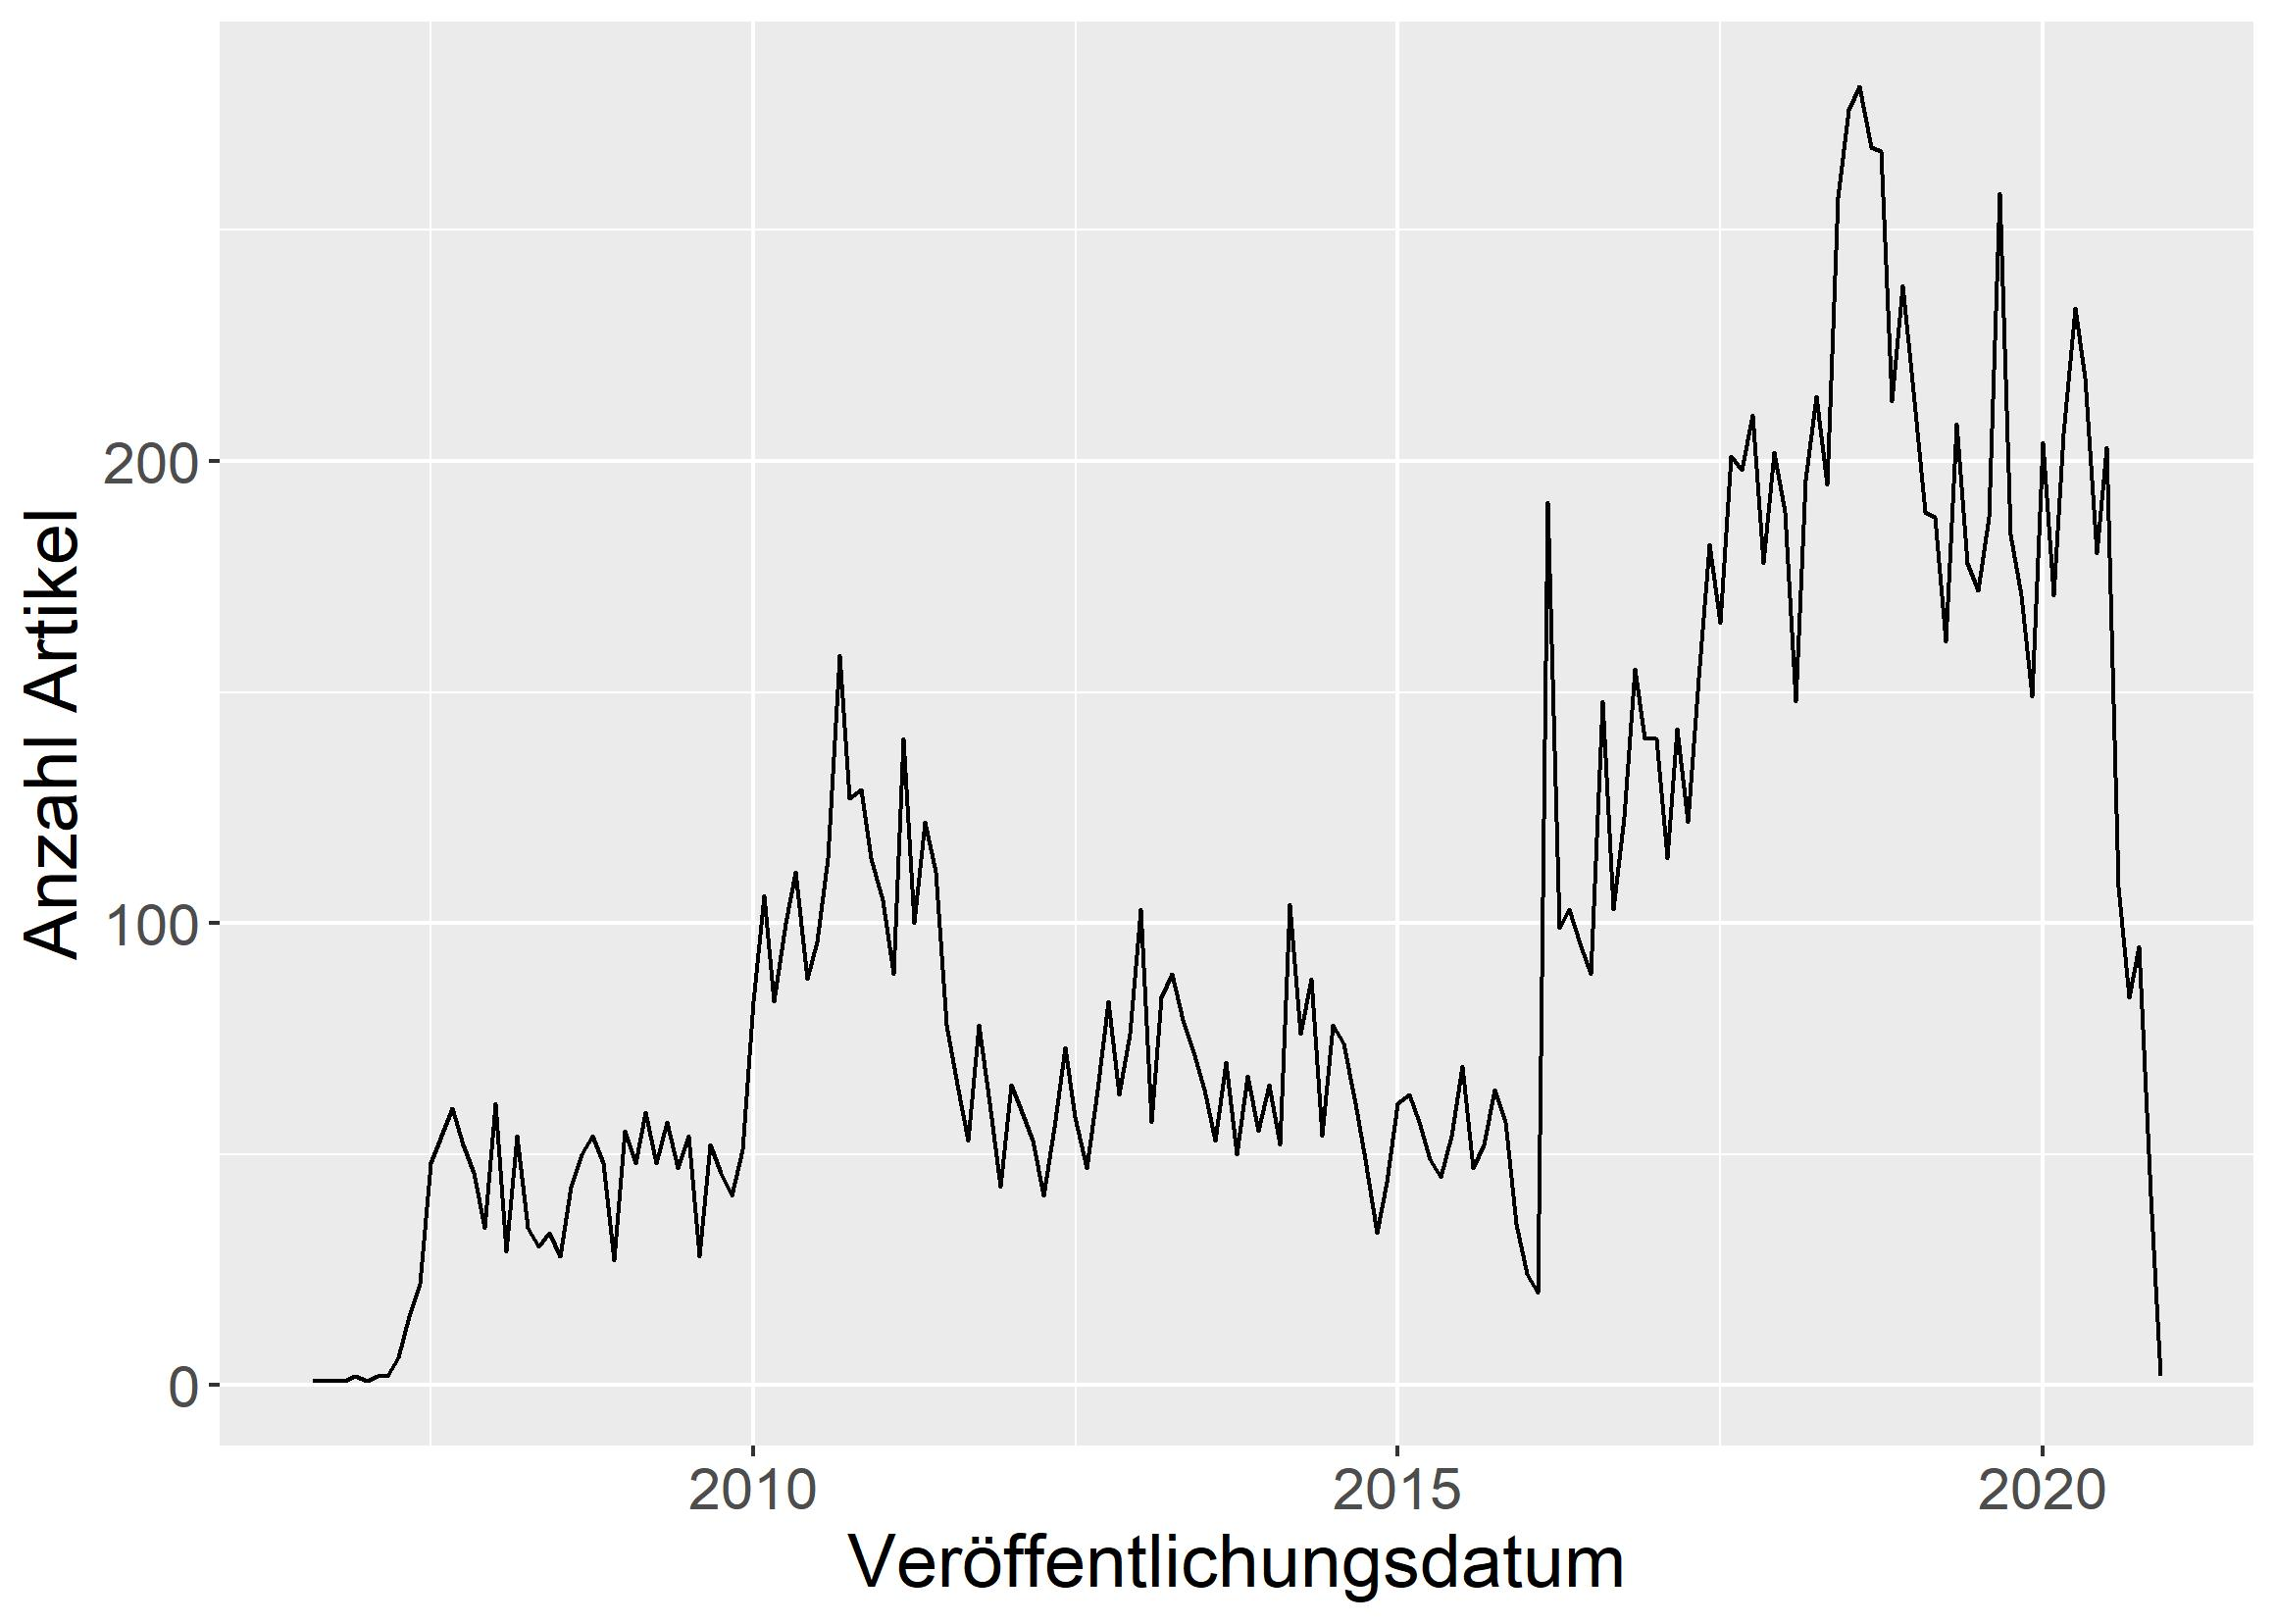
\includegraphics[scale=0.45]{graphics/cons_freq_time.jpg}
    \caption{Anzahl Artikel nach Veröffentlichungsdatum (nach Monat gruppiert)}
    \label{article-frequency}
\end{figure}

Der so erstellte Korpus umfasst insgesamt 16836 Texte und deckt beginnend in 2006 einen Zeitraum von 14 Jahren ab.
Die zeitliche Verteilung der Artikel im Korpus ist Grafik \ref{article-frequency} zu entnehmen, wie dort ersichtlich ist steigt beginnend in 2016 die Zahl der Artikel deutlich an.
Dies ist zum einen damit zu erklären, dass einzelne der gecrawlten Websites ihre Veröffentlichungsfrequenz zu dieser Zeit erhöht haben, überwiegend ist diese Entwicklung aber darauf zurückzuführen, dass insbesondere das Angebote von \textit{Watergate.tv} erst im Jahr 2016 seinen Betrieb aufgenommen hat und eine hohe Veröffentlichungsfrequenz aufweist. 
Genauere Informationen zu den von den einzelnen Angeboten abgedeckten Zeiträumen sowie zu Artikelzahl und Länge finden sich in Tabelle \ref{corpus-stats}.

Ebenso ist dort ersichtlich, dass sich nicht nur die absolute Zahl der Artikel nach Quelle stark unterscheidet, auch das Veröffentlichungsinterval schwankt je nach Quelle von weniger als einem Artikel/Monat zu über 100.
Es besteht weiterhin ein negativer Zusammenhang zwischen der Artikellänge und dem Veröffentlichungsintervall ($r = -0.72, p = 0.065$).

\begin{table}
    \begin{center}
        \begin{tabularx}{\textwidth}{lXXXXX}
            \toprule
            & Von & Bis & Mittlere Zeichenzahl & Anzahl Artikel & Artikel/Monat\\
            \midrule
            Alles Schall und Rauch & 23.08.2006 & 02.08.2020 & 5000 & 5349 & 32.0\\
            conrebbi & 05.09.2012 & 20.10.2014 & 5610 & 24 & 1.0\\
            deutschlandpranger & 29.10.2016 & 30.12.2020 & 7527 & 118 & 2.4\\
            fm-tv & 31.07.2008 & 02.11.2018 & 9158 & 97 & 0.8\\
            hinterderfichte & 16.01.2010 & 31.05.2018 & 4221 & 1083 & 10.8\\
            \addlinespace
            recentr & 03.08.2007 & 05.08.2020 & 5071 & 4762 & 30.5\\
            Watergate.tv & 20.05.2016 & 16.11.2020 & 2810 & 5403 & 101.9\\
            \bottomrule
            \end{tabularx}
        \caption{Kennzahlen der einzelnen Quellen des Korpuses}
        \label{corpus-stats}
    \end{center}
\end{table}

Auch eine inhaltliche Betrachtung zeigt deutliche Unterschiede zwischen den einzelnen Quellen.
So ist \textit{Alles Schall und Rauch} (\textit{ASuR}) als ältestes vertretenes Angebot auch einer der "klassischsten" Vertreter der Verschwörungswebsites.
Hier werden die Besucher:innen direkt auf der Startseite mit Fragen konfrontiert wie \enquote*{Was geschau wirklich am 11. September?} oder \enquote*{Was passiert tatsächlich mit dem Klima?} \parencite{asur-homepage}.
Hier lässt sich bereits die von \textcite[][205]{filatkina_2018} beobachtete Konstruktion des offenen Fragen finden, die die Aufmerksamkeit der Leser:innen auf sich ziehen soll.

Die Seite bedient sich klassischer Verschwörungstheorien und wird im allgemeinen der Truther Szene zugeordnet \parencite{psiram-asur}.
Sie hat laut Eigenaussage im Schnitt über 50.000 Zugriffe täglich.\footnote{Der Besucherzähler der Website ist inzwischen nicht mehr funktional, Angabe übernommen aus \textcite{vice-asur}}

Inhaltlich finden sich sowohl Essay-artige Artikel zu Themen wie 9/11, den Bilderberger-Treffen oder dem Klimawandel auf der Seite, aber auch kürzer gehaltene Meldungen zu aktuellen Ereignissen.
Es werden, wie bei fast allen anderen Seiten im Korpus, häufig Inhalte Dritter eingebunden sowie die Artikel durch Bilder oder Grafiken ergänzt.
Hier lässt sich Bereits die von \textcite{soukup_2008} beobachtete Multimedialität von Verschwörungstheorien beobachten.

Ähnlich zu \textit{ASuR} gelagert sind auch die Websites \textit{Hinter der Fichte} (\textit{HdF}) und \textit{conrebbi}, beide können der Truther Szene zugerechnet werden \cite[siehe etwa][]{psiram-conrebbi}.
In beiden Angeboten werden aktuelle Ereignisse kommentiert und verschwörungstheoretisch interpretiert, aber auch längere Essays zu typischen Themen der Szene verfasst.
Im Vergleich zu \textit{ASuR} werden bei beiden Angeboten deutlich mehr Inhalte in Form von Videos und Fremdquellen in Bild und Textform genutzt.

Von den bisherigen Quellen abheben tun sich dagegen die Angebote \textit{fm-tv} sowie \textit{Deutschlandpranger}.
Während sich beim \textit{Deutschlandpranger} etwa inhaltlich recht klassische Themen wie die Leugnung des Klimawandels \parencite*[vgl.][]{dprang-klima} finden, sind die dazugehörigen Text überdurchschnittlich lang und voller Werbung für Bücher zu z.T. komplett unabhängigen Themen.
Insbesondere aber sind die Texte selbst z.T. sehr wirr, die (sehr ausführlichen) AGB der Website enthalten etwa einen Abschnitt zu Strafzahlungen bei "Übersenden eines Statements anstatt einer echten Rechnung (True Bill) des wahren Haftungsgläubigers" \parencite*{dprang-agb} und weitere ähnlich obskure Paragraphen .

Die verbleibenden beiden Quellen im Korpus \textit{recentr} und \textit{Watergate.tv} sind beide der rechten truther Szene zuzuordnen und verbreiten Verschwörungstheorien in diese Richtung.
Beide zeichnet ein eher journalistischer Stil aus, es werden kurze bis mittellange Meldungen veröffentlicht, häufig begleitet von eigenen oder fremden Videos.
\textit{Recentr} wurde 2006 als deutscher Ableger von \textit{Inforwars.com} gegründet und bedient sich noch heute einem ähnlichen Konzept.
Ähnlich dem Vorbild wird massiv Werbung für den eigenen Shop gemacht in dem diverse Produkte zur Vorbereitung auf apokalyptische Szenarien sowie fragwürdige Nahrungsergänzungsmittel verkauft werden.
Inhaltlich sticht vor allem heraus, dass sich die Seite (bzw. der Hauptautor Alexander Benesch) z.T. sehr explizit von anderen Teilen der rechten/verschwörungstheoretischen Szene abgrenzt.
\footnote{So grenzt sich das Portal in Beiträgen inzwischen auch von \textit{Inforwars} Gründer Alex Jones ab \parencite*{recentr-jones} oder spekuliert darüber, ob die Alternative für Deutschland vom britischen Geheimdienst gegründet wurde \parencite{recentr-afd}}
So kommt es durchaus vor, dass in einem Artikel zunächst von der "implausiblen Sichtweise, verschiedenste Regierungen hätten eine Fake-Pandemie orchestriert" \parencite{recentr-population} gesprochen wird, nur um im nächsten Satz zu erklären: 

\begin{quotation}
    In Wirklichkeit sind die Methoden der globalen Bevölkerungsreduktion fast ausschließlich legal, simpel und werden schrittweise angewandt [...]. Das Konzept ist so entworfen, um mit möglichst wenig Zwang auszukommen [...]. \parencite{recentr-population}
\end{quotation} 

Die Website \textit{Watergate.tv} (inzwischen Teil von \textit{NEOPresse.com}) ist ein Nachrichten und Videoportal, das sich verschwörungstheoretischer Narrative bedient. 
Auf dem Portal finden sich klassische Themen wie Bilderberger-Treffen \parencite[vgl.][]{watergate-bilderberger} aber auch Fake-News und Berichterstattung mit starker pro-russischen Tendenz.
In die öffentlichkeit rückte das Portal als sich das Neo-Magazin-Royale wegen seiner Mitarbeit bei \textit{Watergate.tv} von Hans Meiser trennte \parencite*[Siehe z.B.][]{spiegel-watergate}.

Insgesamt deckt der hier verwendete Korpus einen signifikaten Teil der eher klassischen deutschsprachigen Truther Szene ab.
Es muss allerdings angemerkt werden, dass insbesondere in den letzten Jahren eine Bewegung in der Szene Richtung Social Media zu Portalen wie Facebook und Telegram stattfand.\todo{Eventuell noch ne Zitation reinwamsen.}
Diese zu Untersuchen ist allerdings nicht Teil der Fragestellung dieser Arbeit.

\subsection{Vergleichskorpus}

Um einen möglichst guten Vergleich zwischen den Texten im Korpus und dem Vergleichskorpus zu ermöglichen war es das Ziel Medien zu finden die in Form und inhaltlicher Ausrichtung dem Korpus möglichst ähnlich sind, ohne aber deren verschwörungstheretische Aspekte zu teilen.
Da insbesondere die letzten beiden besprochenen Angebote sich inhaltlich sehr an journalisitsche Angebote anlehnen, lag es nah ebensolche heranzuziehen.
Aus Gründen der Vollständigkeit (die Angebote sollten möglichst den kompletten Zeitraum des Korpus abdecken) sowie der Zugänglichkeit wurden die Angebote von \textit{Spiegel Online} sowie der \textit{Frankfurter Rundschau} ausgewählt.
Es wurde für beide Onlineangebote zunächst ein Index aller Artikel die in den selben Zeitraum wie der Korpus fallen erstellt und aus diesem zufällig eine Auswahl von 10000 Artikeln pro Anbieter gezogen.

Da die restlichen im Korpus enthaltenen Seiten alle mehr oder weniger in der Form eines Blogs gestaltet sind, sollten Angebote vergleichbarer Form herangezogen werden.
Um auch dem in der Literatur häufig genannten wissenschaftlichen Stil von verschwörungstheoretischen Texten Rechnung zu tragen wurde eine Reihe von Wissenschaftsblogs als zweite Komponente im Vergleichskorpus gewählt.
Dafür wurden von den beiden Platformen \textit{scienceblogs} und \textit{scilogs}\footnote{Beide Platformen sind Anbieter bei denen eine Vielzahl verschiedener Blogs zu finden sind.} ähnlich den journalistischen Angeboten aus dem gesamten Index der Einträge eine Auswahl von jeweils 10000 Artikeln ausgewählt.
Genauere Kennwerte zum Vergleichskorpus sind Tabelle \ref{comcorpus-stats} zu entnehmen.

\begin{table}
    \begin{center}
        \begin{tabularx}{\textwidth}{XXXXXX}
            \toprule
            & Von & Bis & Mittlere Zeichenzahl & Anzahl Artikel & Artikel/Monat\\
            \midrule
            Frankfurter Rundschau & 03.08.2006 & 04.08.2020 & 3670 & 9959 & 59.3\\
            scienceblogs & 14.02.2007 & 04.08.2020 & 3261 & 8765 & 54.4\\
            scilogs & 29.12.2000 & 03.08.2020 & 5206 & 9533 & 40.6\\
            Spiegel Online & 01.08.2006 & 07.01.2020 & 4687 & 8665 & 53.8\\
            \bottomrule
        \end{tabularx}
        \caption{Kennzahlen der einzelnen Quellen des Vergleiskorpuses}
        \label{comcorpus-stats}
    \end{center}
\end{table}

\subsection{Datenvorverarbeitung}

Zunächst wurden einige Süberungsverfahren auf den Korpus angewendet, um zu verhindern, dass fehlerhafte oder irrelevante Daten mit für die Feature Erstellung herangezogen werden.

Es wurde zunächst Unicode Normalisierung für alle Texte durchgeführt, anschließend wurde mittels des \textit{Google Compact Language Detector 3} \parencite[][]{cld3} die Sprache aller Text bestimmt und alle überwiegend Fremdsprachigen Artikel wurden aus dem Korpus entfernt.
Da im Korpus an einigen Stellen nicht zum Artikeltext gehörige Komponenten aus vielen Sonderzeichen vorhanden waren, wurden alle Wörter entfernt, die nur aus Zeichen bestanden, die unter 1000 Mal im gesamten Korpus vorhanden waren.
Weiterhin wurden noch kleinere Korrekturen vorgenommen, wie das Zusammenfassen multipler, aufeinanderfolgender Leerzeichen und Unterstriche (die gerne als Trennlinien in den Text benutzt wurden).

Abschließend wurden noch alle Text unter 100 Zeichen Länge aus dem Korpus entfernt, da diese für die Klassifizierungsaufgabe nur wenig Informationen enthalten können. Der finale Korpus umfasste 53758 Texte, mit einem Anteil der positiven Klasse (sprich von verschwörungstheoretischen Texten) von etwa 32\%.

\subsection{Features}

Zunächst wurden Features basierend auf den in der Literatur beobachteten linguistischen Eigenschaften von verschwörungstheoretischen Texten erstellt.
Die etwa von \textcite*[10]{miller_2002} festgestellte Emotionalität wird mit der Methode der Sentimentanalyse bearbeitet.
Dafür wurde das Sentimentwörterbuch \textit{SentiWS} \parencite[][]{sentiws} genutzt.
Dieses umfasst positive und negative Sentimentwerte für über 3000 Grundformen deutscher Wörter.
Während komplexere Ansätze wie etwa der von \textcite[]{ml_sentiment} eine höhere Präzision versprechen,\footnote{So ist der hier vorgestellte Ansatz nicht in der Lage korrekt mit Negationen umzugehen.} scheint die genutzte Methode für den vorliegenden Kontext ausreichende Ergebnisse zu lieferen.
Es wurde sowohl die Summe der positiven und negativen Sentimente erfasst, also auch die Summe sowie der Betrag nach Text insgesamt.
Hiermit soll insbesondere auf solche Fälle eingegangen werden, in denen ein Text zwar viele emotional behaftete Wörter verwendet, sich die Sentimentsumme aber durch einen Wechsel an positiven und negativen Wörtern ausgleicht.

Als weiteres in der Literatur anzutreffendes Merkmal soll auch die Menge an Zitationen betrachtet werden.
Um diese zu operationalisieren wurden zum einen die Anzahl der Anführungszeichen im Text gezählt.
Eine genauere Betrachtung der Verwendung von Fremdbelegen von denen etwa \textcite[235]{schafer_2018} spricht, wird ermöglicht indem als zusäztliche Features erfasst werden:
\begin{enumerate}
    \item Die Zahl der äußersten Zitate\footnote{Also Zitate die nicht Teil anderer Zitate sind}
    \item Die durchschnittliche Länge der Zitate
    \item Der Anteil von zitiertem Text am gesamten Artikeltext
\end{enumerate}

Die Menge an \textit{scare quotes} wird ebenfalls erfasst, wobei ein \textit{scare quote} für diese Arbeit definiert wird als ein Zitat in dem keine Leerzeichen (oder andere Formen von whitespaces) enthalten sind.

Die Menge der Fragen, wie sie etwa \textcite[205]{filatkina_2018} als Merkmal von verschwörungstheoretischen Texten feststellt, wird durch ein simples Zählen der im Text vorkommenen Fragezeichen abgebildet.
Ähnlich lässt sich auch die Annahme über die Häufung von Zahlenangaben wie sie sich bei \textcite[234]{schafer_2018} findet, durch einfaches Zählen von Zahlengruppen operationalisieren.
Um die bei \textcite[149]{stumpf_2019} gemachte Beobachtung der häufigen Verwendung von Negationswörtern abzubilden, wurde händisch eine Liste von 15 Negationswörtern erstellt und deren Häufigkeit in den Texten gemessen.

Die Multimedialität und Verknüpftheit von Verschwörungstheoretischen Online Texten wie sie \textcite[10]{soukup_2008} anspricht soll mit einer Reihe von Informationen die aus den dem Korpus zugrunde liegenden HTML Dateien extrahiert wurden abgebildet werden.
Um die Multimedialität zu erfassen wurde die Anzahl der eingebundenen Bilder, Tweets, Youtube-Videos sowie sonstiger eingebetteter Elemente im Artikel gezählt.
Für eine Messung der Verknüpftheit wurde die Anzahl von in den Artikeln enthaltenen Links, aufgeteilt nach internen und externen Zielen, erfasst.
Ebenso wurde als stilistisches Merkmal die Menge an fettgedruckten und kursiven Text erfasst.

\begin{table}
    \begin{center}
        \begin{tabularx}{\textwidth}{XXXXXXX}
            \toprule
            Feature & \multicolumn{2}{X}{Korpus} & \multicolumn{2}{X}{Vergleichskorpus} & W & p\\
            & $\overline{X}$ & $\sigma$ & $\overline{X}$ & $\sigma$ & & \\
          \midrule
          Textlänge & 4309 & 4429 & 4208 & 4186 & \num{3.01e8} & $<0.01$\\
          Tweets & 0.0006 & 0.0058 & 0.0004 & 0.013 & \num{3.13e8} & $<0.01$\\
          Youtube-Videos & 0.016 & 0.088 & 0.004 & 0.037 & \num{3.45e8} & $<0.01$\\
          Interne Links & 0.0094 & 0.066 & 0.077 & 0.274 & \num{2.31e8} & $<0.01$\\
          Externe Links & 0.081 & 0.2 & 0.12 & 0.434 & \num{3.16e8} & $<0.01$\\
          \addlinespace
          Negationen & 0.158 & 0.11 & 0.151 & 0.109 & \num{3.23e8} & $<0.01$\\
          Anteil Zitation & 9.351 & 18.062 & 7.373 & 13.984 & \num{2.91e8} & $<0.01$\\
          Sentimente Betrag & 8.778 & 9.615 & 7.649 & 8.039 & \num{3.15e8} & $<0.01$\\
          \bottomrule
        \end{tabularx}
        \caption{Statistische Kennzahlen zu ausgewählten Features}
        \label{feature-stats}
    \end{center}
\end{table}

Um weitere Features aus dem Bereich der Textklassifikation zu nutzen, wurde der Corpus zunächst mithilfe von \textit{spaCy} \parencite[][]{spacy} annotiert um Lemmata und Part-of-Speech Tags zu generieren.
Es wurden anschließend die Anzahl jedes Part-of-Speech Tags sowie der Anteil an großgeschriebenen Text und Sonderzeichen als Feature übernommen.
Ebenso wurde die Wortdichte für jeden Text bestimmt, also die Anzahl an Wörtern im Verhältnis zur Textlänge.

Zur Ermittlung von Wortfrequenzen wurden zunächst Stopwörter aus dem Corpus entfernt\footnote{Zum Einsatz kam die Stopwort Liste aus dem \textit{tm} Paket \parencite[][]{r-tm}}, Wörter auf ihre Lemmata reduziert, einige Sonderfälle aussortiert\footnote{So wurde beispielsweise das Wort dpa nicht übernommen, da es praktisch exklusiv in Artikeln der Frankfurter Rundschau und von Spiegel Online vorkommt.} und anschließend die 400 häufigsten Wörter als Features übernommen.\footnote{Es ist durchaus üblich mehr Wörter als Features zu übernehmen \parencite*[siehe etwa][68]{feldman_sanger_2006}, da dies aber die Dimensionalität der Daten und damit die Komplexität der Klassifizierung deutlich erhöhen würde und die Auswahl von 400 Wörtern bereits zufriedenstellende Ergebnisse liefert wurde hier darauf verzichtet.}
Alle Features abgesehen von den sowieso als \textit{tf-idf} oder als relative Häufigkeit vorliegenden wurden mit der Textlänge skaliert.

\subsection{Modelerstellung}

Zunächst wurde ein Datensatz erstellt der alle Beobachtungen, aber nur solche Features enthielt die aus der Literatur zu Verschwörungstheorien abgeleitet wurden.
Auf diesem Datensatz wurde zunächst ein einfacher Entscheidungsbaum aus dem Paket \textit{rpart} \parencite[]{rpart} als Baseline Klassifizierer trainiert.
Hierfür wurde ein Train/Test Split im Verhältnis 2/1 auf den Daten durchgeführt.
Das auf den Trainingsdaten trainierte Modell erreichte eine Präzision von 75.3\%.


\begin{table}
    \begin{center}
        \begin{tabularx}{\textwidth}{XXXXX}
            \toprule
            Modell & Accuracy & Sensitivity & Specificity & AUC\\
            \midrule
            dtree & 0.7534 & 0.7761 & 0.7428 & 0.829445 \\
            lightGBM & 0.8745 & 0.8700 & 0.8766 & .0.950817 \\
            \bottomrule
        \end{tabularx}
        \caption{Ergebnisse der Klassifizierer nur auf literaturbasierten Features}
        \label{small-model}
    \end{center}
\end{table}


Mit dem gleichen Daten wurde anschließend ein Modell mit der \textit{LightGBM} Bibliothek\parencite[][]{lightgbm} trainiert.
Da Gradienten-Boosting Verfahren schnell zu Overfitting neigen wurde dafür zunächst mittels Kreuzvalidierung auf den Trainingsdaten die optimale Iterationstiefe bestimmt.
Anschließend wurde das Modell mit einer Lernrate von 0.1 und einer maximalen Blattzahl von 50 trainiert.
Das so trainierte Modell erreichte eine Präzision von 87.4\%.

In Tabelle \ref{small-model} sind die Leistungen der beiden Modelle auf den Testdaten zusammengefasst.
Wie zu erkennen ist, ist selbst der einfache Entscheidungsbaum deutlich Präziser als es ein bloßes Raten im Klassenverhältnis wäre ($p < 0.01$).
Auch ist ersichtlich, dass das komplexere \textit{LightGBM} Modell eine in allen Bereichen deutlich bessere Klassifizierungsleistung erbringt.

\begin{table}
    \begin{center}
        \begin{tabularx}{\textwidth}{XXXXX}
            \toprule
            Modell & Accuracy & Sensitivity & Specificity & AUC\\
            \midrule
            dtree & 0.8771 & 0.7941 & 0.9158 & 0.901061 \\
            lightGBM (10-Fold Kreuzvalidierung) & 0.9814 & 0.9781 & 0.9828 & N/A \\
            \bottomrule
        \end{tabularx}
        \caption{Ergebnisse der Klassifizierer auf dem vollständigen Datensatz}
        \label{full-model}
    \end{center}
\end{table}

Im weiteren wurde ein Modell mit allen vorhandenen Features erstellt.
Hierfür wurde ebenfalls zunächst ein Baseline Entscheidungsbaum trainiert.
Dieser erreichte eine Präzision von 87.7\% und konnte damit den Entscheidungsbaum der auf dem kleineren Korpus trainiert wurde in Genauigkeit deutlich übertreffen.
Interessant ist vor allem die verhältnismäßig geringe Sensitivität.

Bevor das finale Modell trainiert wurde, wurde zunächst mittels eines Tunegrids eine optimierung der Hyperparameter der Lernrate sowie der Anzahl der äußersten Blätter durchgeführt.
Getestete Werte waren dabei für die Lernrate 0.01, 0.05, 0.10, 0.20 und für die Blätterzahl 5, 50, 127 (Der Standardwert von lightGBM), 200.
Das beste Ergebnis wurde mit einer Lernrate von 0.05 und einer Blätterzahl von 50 erzielt.
Mit diesen Werten wurde erneut die optimale Iterationstiefe mittels Kreuzvalidierung bestimmt.
Das mit diesen Parametern erstellte, finale Modell wurde schließlich mittels einer 10-Fold Kreuzvalidierung validiert und erreichte insgesamt eine Präzision von 98.14\%.


\begin{table}
    \begin{center}
        \begin{tabularx}{\textwidth}{XXXX}
            \toprule
            & & \multicolumn{2}{X}{Referenz}\\
            & & 0 & 1 \\
            \multirow{2}{*}{Vorhersage} & 0 & 33288 & 368 \\
            & 1 & 634 & 16468 \\\midrule
        \end{tabularx}
        \caption{Confusion-Table des finalen Modells}
        \label{confusion-table}
    \end{center}
\end{table}
%TODO: evtl. kurz drauf eingehen


% Ergebnisse

\section{Ergebnisse}

% Fazit

\section{Fazit}

Es wurde, basierend auf einem Korpus aus Artikeln deutschsprachiger, verschwörungstheoretischer Internetangebote und einem Vergleichskorpus aus journalistischen Artikeln, ein Modell trainiert, dass zuverlässig die verschwörungstheoretischen Texte identifizieren kann.

In der Literatur gemachte Beobachtungen zur literarischen Form von Verschwörungstheorien wurden dabei aufgegriffen und als Features in das Modell eingebracht.
Diese leisteten einen wichtigen Beitrag für die Funktion des trainierten Modells.
Es konnte so gezeigt werden, dass einige dieser qualitativen Beobachtungen auch für eine quantitative Analyse von Verschwörungstheorien geeignet sind.
Es wurden weiterhin Wortfrequenzen und Part-of-Speech Tags als zusätzliche Features in das Modell eingebracht.
Das so entstandene Modell arbeitet deutlich genauer.

Der vorgestellte Ansatz konnte eine gute Leistung erbringen, ist dabei aber deutlich weniger komplex als die bisherigen Verfahren zur automatischen Verarbeitung von Verschwörungstheorien.
Er ist dafür allerdings auch deutlich unschärfer, es wird keine spezifische verschwörungstheoretische Aussage erkannt wie dies etwa \textcite[]{samory_2018} tun, vielmehr wird ein verschwörungstheoretischer Stil identifiziert.

Ein mögliches Problem des vorgestellten Verfahrens könnte auch die Generalisierbarkeit des trainierten Modells sein.
Um hier Verbesserungen herbeizuführen wäre die Zusammenstellung eines bedeutend größeren und diverseren Korpuses, sowie auch eines entsprechend Vergleichskorpuses ein sinnvoller Ansatzpunkt.
Auch bedarf es deutlich mehr an quantitativer Grundlagenarbeit zu sprachlichen Eigenschaften von Verschwörungstheorien, um mehr automatisiert verarbeitbare Merkmale zu identifizieren.

Die vorgestellte Arbeit konnte zeigen, dass auch verhältnismäßig einfache Ansätze zur automatischen Erkennung von Verschwörungstheorien grundsätzlich erfolgsversprechend sind und könnte so gut als Startpunkt für weitere Arbeiten in diese Richtung dienen.

\clearpage

%
% ---- Bibliography ----
%
%
\setcounter{biburllcpenalty}{7000}
\setcounter{biburlucpenalty}{8000}

\printbibliography[title=Literatur, keyword=literature]
\printbibliography[title=Software, keyword=software]
\printbibliography[title=Online, keyword=online]

\clearpage

% Die eidesstattliche Erklärung mit Unterschrift
\textbf{Erklärung der Urheberschaft}

\vspace{1cm}

Hiermit erkläre ich, daß ich die vorliegende Arbeit
selbstständig angefertigt, nicht anderweitig zu Prüfungszwecken vorgelegt und
keine anderen als die angegebenen Hilfsmittel verwendet habe. Sämtliche 
wissentlich verwendete Textausschnitte, Zitate oder Inhalte anderer Verfasser 
wurden ausdrücklich als solche gekennzeichnet.

\vfill

\hspace{2cm} Ort, Datum \hfill Unterschrift \hspace{2cm}


\end{document}
